\subsection{The tenant type enumeration type}
\label{sec:application:building_the_model:the_tenant_type_enumeration_type}

In the eleventh step, another enumeration type is introduced. This time, the $.\type{TenantType}$ enumeration type used to specify a type for a tenant is introduced. \cref{subsec:library_of_transformations:type_level_transformations:enumeration_types} is used to introduce the enumeration type on the type level, while on the instance level, \cref{subsec:library_of_transformations:instance_level_transformations:enumeration_values} is used to introduce the values of the enumeration.

The $name$ of the new enumeration type is $.\type{TenantType}$, and it has $values = \{\type{REGULAR}, \type{SUBTENANT}\}$. Please note that there are multiple encodings possible to encode an enumeration type in GROOVE. This time, the encoding using nodes is chosen. The function $fob$ which maps the enumeration values to internal node ids is defined as follows:
\begin{align*}
    fob = \{&(\type{REGULAR}, \text{RegularType}), (\type{SUBTENANT}, SubtenantType)\}
\end{align*}

The function $fid$ which maps the enumeration values to explicit node identifiers is equal to the definition of $fob$, so $fid = fob$. The following model is obtained:

\LTXtable{\textwidth}{tex/06_application/02_building_the_model/tables/11_the_tenant_type_enumeration_type.tex}

\begin{figure}[p]
    \centering
    \begin{subfigure}{0.98\textwidth}
        \centering
        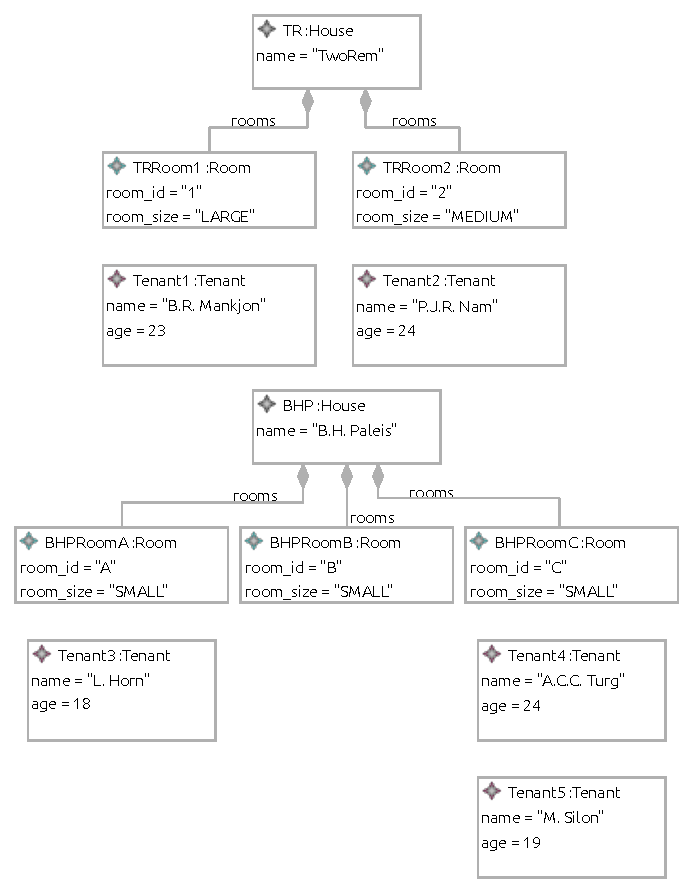
\includegraphics{images/06_application/instance_model/step11.pdf}
        \caption{Instance Model $Im_{11}$}
        \label{fig:application:building_the_model:the_tenant_type_enumeration_type:ecore:instance_model}
    \end{subfigure}
    \\
    \begin{subfigure}{0.98\textwidth}
        \centering
        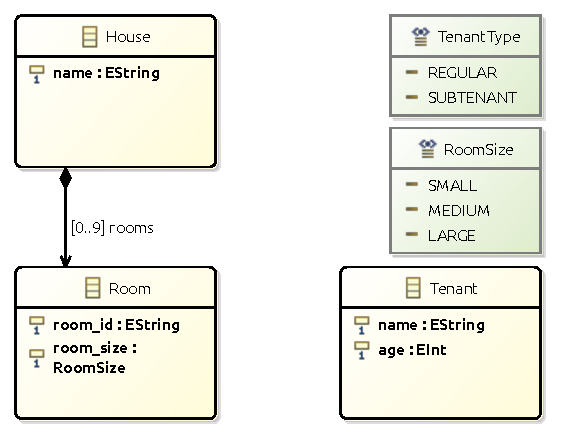
\includegraphics{images/06_application/type_model/step11.pdf}
        \caption{Type Model $Tm_{11}$}
        \label{fig:application:building_the_model:the_tenant_type_enumeration_type:ecore:type_model}
    \end{subfigure}
    \caption{The Ecore model after step 11}
    \label{fig:application:building_the_model:the_tenant_type_enumeration_type:ecore}
\end{figure}

\begin{figure}[p]
    \centering
    \begin{subfigure}{0.98\textwidth}
        \centering
        % To use this figure in your LaTeX document
% import the package groove/resources/groove2tikz.sty
%
\begin{tikzpicture}[scale=\tikzscale,name prefix=step11-]
\node[basic_node] (n0) at (2.825, -6.365) {\ml{\uline{\textit{BHP}} : \textbf{House}\\name = "B.H. Paleis"}};
\node[basic_node] (n1) at (2.655, -0.335) {\ml{\uline{\textit{TR}} : \textbf{House}\\name = "TwoRem"}};
\node[basic_node] (n2) at (2.575, -3.405) {\ml{\uline{\textit{RegularType}} : \textbf{TenantType\$REGULAR}}};
\node[basic_node] (n3) at (5.180, -1.965) {\ml{\uline{\textit{SubtenantType}} : \textbf{TenantType\$SUBTENANT}}};
\node[basic_node] (n4) at (2.845, -4.230) {\ml{\uline{\textit{SmallSize}} : \textbf{RoomSize}\\\textit{SMALL}}};
\node[basic_node] (n5) at (4.405, -0.570) {\ml{\uline{\textit{MediumSize}} : \textbf{RoomSize}\\\textit{MEDIUM}}};
\node[basic_node] (n6) at (0.990, -0.550) {\ml{\uline{\textit{LargeSize}} : \textbf{RoomSize}\\\textit{LARGE}}};
\node[basic_node] (n7) at (1.815, -1.465) {\ml{\uline{\textit{TRRoom1}} : \textbf{Room}\\room\_id = "1"}};
\node[basic_node] (n8) at (3.405, -1.475) {\ml{\uline{\textit{TRRoom2}} : \textbf{Room}\\room\_id = "2"}};
\node[basic_node] (n9) at (1.805, -2.475) {\ml{\uline{\textit{Tenant1}} : \textbf{Tenant}\\age = 23\\name = "B.R. Mankjon"}};
\node[basic_node] (n10) at (3.405, -2.475) {\ml{\uline{\textit{Tenant2}} : \textbf{Tenant}\\age = 24\\name = "P.J.R. Nam"}};
\node[basic_node] (n11) at (0.945, -4.285) {\ml{\uline{\textit{Tenant3}} : \textbf{Tenant}\\age = 18\\name = "L. Horn"}};
\node[basic_node] (n12) at (4.735, -4.225) {\ml{\uline{\textit{Tenant4}} : \textbf{Tenant}\\age = 24\\name = "A.C.C. Turg"}};
\node[basic_node] (n13) at (4.825, -3.275) {\ml{\uline{\textit{Tenant5}} : \textbf{Tenant}\\age = 19\\name = "M. Silon"}};
\node[basic_node] (n14) at (0.910, -5.225) {\ml{\uline{\textit{BHPRoomA}} : \textbf{Room}\\room\_id = "A"}};
\node[basic_node] (n15) at (2.870, -5.215) {\ml{\uline{\textit{BHPRoomB}} : \textbf{Room}\\room\_id = "B"}};
\node[basic_node] (n16) at (4.810, -5.225) {\ml{\uline{\textit{BHPRoomC}} : \textbf{Room}\\room\_id = "C"}};

\path[basic_edge] (n14)  -- node[lab] {\ml{room\_size}} (n4) ;
\path[basic_edge] (n0)  -- node[lab] {\ml{rooms}} (n16) ;
\path[basic_edge](n15.north -| 2.845, -4.230) -- node[lab] {\ml{room\_size}} (n4) ;
\path[basic_edge] (n16)  -- node[lab] {\ml{room\_size}} (n4) ;
\path[basic_edge] (n1)  -- node[lab] {\ml{rooms}} (n8) ;
\path[basic_edge] (n0)  --  (n14) 
node[lab] at (1.960, -5.790) {\ml{rooms}};
\path[basic_edge] (n8)  -- node[lab] {\ml{room\_size}} (n5) ;
\path[basic_edge](n0.north -| 2.870, -5.215) -- node[lab] {\ml{rooms}} (n15) ;
\path[basic_edge] (n7)  -- node[lab] {\ml{room\_size}} (n6) ;
\path[basic_edge] (n1)  -- node[lab] {\ml{rooms}} (n7) ;
\end{tikzpicture}

        \caption{Instance Graph $IG_{11}$}
        \label{fig:application:building_the_model:the_tenant_type_enumeration_type:groove:instance_graph}
    \end{subfigure}
    \\
    \begin{subfigure}{0.98\textwidth}
        \centering
        % To use this figure in your LaTeX document
% import the package groove/resources/groove2tikz.sty
%
\begin{tikzpicture}[scale=\tikzscale,name prefix=step11-]
\node[basic_node] (n0) at (2.825, -6.365) {\ml{\uline{\textit{BHP}} : \textbf{House}\\name = "B.H. Paleis"}};
\node[basic_node] (n1) at (2.655, -0.335) {\ml{\uline{\textit{TR}} : \textbf{House}\\name = "TwoRem"}};
\node[basic_node] (n2) at (2.575, -3.405) {\ml{\uline{\textit{RegularType}} : \textbf{TenantType\$REGULAR}}};
\node[basic_node] (n3) at (5.180, -1.965) {\ml{\uline{\textit{SubtenantType}} : \textbf{TenantType\$SUBTENANT}}};
\node[basic_node] (n4) at (2.845, -4.230) {\ml{\uline{\textit{SmallSize}} : \textbf{RoomSize}\\\textit{SMALL}}};
\node[basic_node] (n5) at (4.405, -0.570) {\ml{\uline{\textit{MediumSize}} : \textbf{RoomSize}\\\textit{MEDIUM}}};
\node[basic_node] (n6) at (0.990, -0.550) {\ml{\uline{\textit{LargeSize}} : \textbf{RoomSize}\\\textit{LARGE}}};
\node[basic_node] (n7) at (1.815, -1.465) {\ml{\uline{\textit{TRRoom1}} : \textbf{Room}\\room\_id = "1"}};
\node[basic_node] (n8) at (3.405, -1.475) {\ml{\uline{\textit{TRRoom2}} : \textbf{Room}\\room\_id = "2"}};
\node[basic_node] (n9) at (1.805, -2.475) {\ml{\uline{\textit{Tenant1}} : \textbf{Tenant}\\age = 23\\name = "B.R. Mankjon"}};
\node[basic_node] (n10) at (3.405, -2.475) {\ml{\uline{\textit{Tenant2}} : \textbf{Tenant}\\age = 24\\name = "P.J.R. Nam"}};
\node[basic_node] (n11) at (0.945, -4.285) {\ml{\uline{\textit{Tenant3}} : \textbf{Tenant}\\age = 18\\name = "L. Horn"}};
\node[basic_node] (n12) at (4.735, -4.225) {\ml{\uline{\textit{Tenant4}} : \textbf{Tenant}\\age = 24\\name = "A.C.C. Turg"}};
\node[basic_node] (n13) at (4.825, -3.275) {\ml{\uline{\textit{Tenant5}} : \textbf{Tenant}\\age = 19\\name = "M. Silon"}};
\node[basic_node] (n14) at (0.910, -5.225) {\ml{\uline{\textit{BHPRoomA}} : \textbf{Room}\\room\_id = "A"}};
\node[basic_node] (n15) at (2.870, -5.215) {\ml{\uline{\textit{BHPRoomB}} : \textbf{Room}\\room\_id = "B"}};
\node[basic_node] (n16) at (4.810, -5.225) {\ml{\uline{\textit{BHPRoomC}} : \textbf{Room}\\room\_id = "C"}};

\path[basic_edge] (n14)  -- node[lab] {\ml{room\_size}} (n4) ;
\path[basic_edge] (n0)  -- node[lab] {\ml{rooms}} (n16) ;
\path[basic_edge](n15.north -| 2.845, -4.230) -- node[lab] {\ml{room\_size}} (n4) ;
\path[basic_edge] (n16)  -- node[lab] {\ml{room\_size}} (n4) ;
\path[basic_edge] (n1)  -- node[lab] {\ml{rooms}} (n8) ;
\path[basic_edge] (n0)  --  (n14) 
node[lab] at (1.960, -5.790) {\ml{rooms}};
\path[basic_edge] (n8)  -- node[lab] {\ml{room\_size}} (n5) ;
\path[basic_edge](n0.north -| 2.870, -5.215) -- node[lab] {\ml{rooms}} (n15) ;
\path[basic_edge] (n7)  -- node[lab] {\ml{room\_size}} (n6) ;
\path[basic_edge] (n1)  -- node[lab] {\ml{rooms}} (n7) ;
\end{tikzpicture}

        \caption{Type Graph $TG_{11}$}
        \label{fig:application:building_the_model:the_tenant_type_enumeration_type:groove:type_graph}
    \end{subfigure}
    \caption{The GROOVE graphs after step 11}
    \label{fig:application:building_the_model:the_tenant_type_enumeration_type:groove}
\end{figure}

A visual representation of $Tm_{11}$ and $Im_{11}$ can be found in \cref{fig:application:building_the_model:the_tenant_type_enumeration_type:ecore}. Similarly, a visual representation of $TG_{11}$ and $IG_{11}$ can be found in \cref{fig:application:building_the_model:the_tenant_type_enumeration_type:groove}. Please note that because of the definitions of $f_{11}(Im_{11})$ and $f'_{11}(IG_{11})$, we have that $f_{11}(Im_{11}) = IG_{11}$ and $f'_{11}(IG_{11}) = Im_{11}$. Furthermore, $f_{11}(Im_{11})$ and $f'_{11}(IG_{11})$ are valid mapping functions themselves, such that they can be combined with another mapping function in the next step.

The introduction of the tenant type enumeration type shows how different encodings can be combined within the transformation framework. The previous enumeration for room sizes was encoded using flags, while this enumeration is encoded using nodes types. Both of these encodings are present in the same model with the same transformation function.

\afterpage{\FloatBarrier}